\documentclass[../sparc.tex]{subfiles}
\graphicspath{{\subfix{../images/}}}
\begin{document}

%%%%%%%%%%%%%%%%%%%%%%%%%%%%%%%%%%%%%%%%%%%%%%%%%%%%%%%%%%%%%%%%%%%%%%%%%%%%%%%%
\section{Wokwi Simulator}

To program an Arduino you don't have to have a real Arduino board -- you can use
a \emph{simulator} instead.  The goal of a simulator is to imitate a real system
with minimal differences from the original.

By the way, there are two similar terms: \emph{simulator} and \emph{emulator}.

Let's look at the differences\cite{so:simulator-vs-emulator} between those two
terms:

\begin{itemize}
\item The task of an \emph{emulator} is to imitate the outer observable behavior
  of a system.  The state of inner workings of an emulation does not have to
  mirror the internal state of an emulated system.
\item The task of a \emph{simulator} is to model the internal state of a
  simulated system.  The end result of a good simulation is a model that
  duplicates the target system in the smallest details.  In an ideal case we
  have to be able to look inside a simulation and observe all the aspects of
  inner workings that we could observe in the same situation inside a simulated
  object.
\end{itemize}

Simulators can be divided between three categories:
\begin{itemize}
\item \emph{Offline simulators} are standalone programs that we can download,
  install and run on a computer.
\item \emph{Online simulators} are special web sites (or rather web
  applications) that allow us to simulate a hardware platform inside a web
  browser (either by downloading all the required code inside a browser or by
  doing some operations on a server.)
\item \emph{Composite simulators} are standalone programs that however require
  an Internet connection to a server to run.
\end{itemize}

Online simulators are easier for beginners as they don't require installation to
a computer.  However many of such simulators require registration which is not
acceptable for some users.

One of the free-access simulators that does not require registration is the
Wokwi project (\href{https://wokwi.com/}{wokwi.com}.)  This simulator allows us
to work not only with the Arduino platform but also with other micro-controllers
(such as STM32 and ESP) and with single-board computers.

Wokwi allows us quite easily to build Arduino projects, program and run them.

One of the key parameters of a simulator is the speed -- the faster a simulator
works, the closer to the simulated hardware platform will be the speed of a
running project.  The speed of the Wokwi online-simulator depends on the
performance of a computer, the type of a web-browser and the complexity of the
built schematics.

The most optimal web-browser for working with Wokwi is Google Chrome or
Chromium, but Mozilla Firefox performs comparatively well too.

Wokwi has context documentation for different electronic components that we can
use in our schematics.

One of the limitations of Wokwi (at the time of writing of this section) is the
simulation speed inconsistency which negatively impacts projects that require
stable (real-time) response time (e.g. projects that working with sound.)

%%%%%%%%%%%%%%%%%%%%%%%%%%%%%%%%%%%%%%%%%%%%%%%%%%%%%%%%%%%%%%%%%%%%%%%%%%%%%%%%
\subsection{First Steps}

To start working with Arduino we have to select ``Arduino (Uno, Mega, Nano)'' on
the main Wokwi page, in the ``Simulate with Wokwi Online'' section.  Then we
have to scroll down the page to the ``Start from Scratch'' section and select
the desired variant of the Arduino.

After that a page will be opened, where we can find the source code editor (akin
to Arduino IDE) on the left and the schematics editor on the right.  The green
button with ``>'' icon on the top left corner of the schematics editor allows us
to run the project in the simulator.  ``+'' button allows us to select and add
components into our schematics, and the button with three dots on it allows us
to access the simulator options.

%%%%%%%%%%%%%%%%%%%%%%%%%%%%%%%%%%%%%%%%%%%%%%%%%%%%%%%%%%%%%%%%%%%%%%%%%%%%%%%%
\newpage
\subsection{Components for building circuits}

\begin{longtable}{|>{
      \centering\arraybackslash
    }p{3cm}|>{
      \centering\arraybackslash}p{8cm}|
  }
  \hline
  Image & Description \\ \hline
  \endfirsthead

  \hline
  Image & Description \\ \hline
  \endhead

  \hline
  \parbox[t][1.4cm][c]{2cm}{\centering \vspace{1cm}
    
\includegraphics[width=0.12\textwidth]{wokwi/wokwi-led.png}} &
  \parbox[t][3cm][t]{8cm}{
    \centering \textbf{Light-emitting diode (LED)}\\ \raggedright

    An LED has two legs: the long one (``+'', an anode), that should be connected
    to an Arduino through a resistor and a short one (``-'', a cathode) that
    should be connected to the ground (GND.)  A resistor is required as without
    it an LED can overheat and burn out as well as the Arduino board itself.

  } \\  \hline

  \parbox[t][0,5cm][c]{2cm}{\centering \vspace{1cm}
    
\includegraphics[width=0.12\textwidth]{wokwi/wokwi-resistor.png}} &
  \parbox[t][2.6cm][t]{8cm}{
    \centering \textbf{Resistor}\\ \raggedright

    A resistor is a component that limits the electric current in a circuit and
    keeps other components from an overload.  It is used to control the electric
    current, to lower the voltage and thus for keeping other components from
    burning out.

  } \\  \hline

  \parbox[t][2,3cm][c]{2cm}{\centering \vspace{0.8cm}
    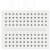
\includegraphics[width=0.12\textwidth]{wokwi/wokwi-breadboard.png}} &
  \parbox[t][3.9cm][t]{8cm}{
    \centering \textbf{Breadboard}\\ \raggedright

    A breadboard is a tool that allows us to quickly and conveniently build
    electric circuits without the need of soldering.  It consists of a sequence
    of ports connected with conductive lines.

  } \\  \hline

  \parbox[t][3,6cm][c]{2cm}{\centering \vspace{1cm}
    
\includegraphics[width=0.12\textwidth]{wokwi/wokwi-rgb-led.png}} &
  \parbox[t][5.1cm][t]{8cm}{
    \centering \textbf{RGB light-emitting diode (LED)}\\ \raggedright

    An RGB LED is in fact three separate LEDs packed in one package, each one is
    of different color: red, green and blue.  We can combine those colors to get
    new color variants.  Usually an RGB LED has 4 legs: one leg is for common
    anode (``+'') or cathode (``-''), and one leg for each color.  Each one of
    color legs should be connected to an Arduino through a resistor to limit the
    electric current, as with the regular LEDs.

  } \\  \hline

  \parbox[t][2,8cm][c]{2cm}{\centering \vspace{1cm}
    
\includegraphics[width=0.12\textwidth]{wokwi/wokwi-lcd2004.png}} &
  \parbox[t][4.3cm][t]{8cm}{
    \centering \textbf{Alphanumeric LCD}\\ \raggedright

    An alphanumeric LCD is a display that allows us to show textual information
    using liquid crystals.  It consists of a set of pixels, that can be enabled
    or disabled to draw symbols.  To connect an LCD display to an Arduino we can
    use several pins: two pins to transfer the data (SDA and SCL) and two pins
    for power (VCC and GND.)

  } \\  \hline

  \parbox[t][2,5cm][c]{2cm}{\centering \vspace{1cm}
    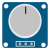
\includegraphics[width=0.12\textwidth]{wokwi/wokwi-potentiometer.png}} &
  \parbox[t][4.3cm][t]{8cm}{
    \centering \textbf{Potentiometer}\\ \raggedright

    A potentiometer is a variable resistor that allows us to change its
    resistance, and that in turn provides us with the ability to control
    different parameters of our systems (brightness, sound volume, speed etc.)
    Usually it has three pins: two for connecting power and ground and the
    middle pin for connecting to analog inputs on an Arduino.  By turning the
    potentiometer handle we can change the resistance between the middle pin and
    the other ones.

  } \\  \hline

  \parbox[t][1,8cm][c]{2cm}{\centering \vspace{1cm}
    
\includegraphics[width=0.12\textwidth]{wokwi/wokwi-buzzer.png}} &
  \parbox[t][3.6cm][t]{8cm}{
    \centering \textbf{Buzzer}\\ \raggedright

    A buzzer (or speaker) is a component that allows us to play sounds by
    sending electric signals to it.  It has two pins: ``+'' should be connected
    to an Arduino digital pin (configured in \texttt{OUTPUT} mode) and ``-'' pin
    that should be connected to the ground (GND.)

  } \\  \hline

  \caption{Some components that are available in Wokwi.}
\end{longtable}

\end{document}
